    \section{Test Stand Description}
    \subsection{Global Requirements and Constraints}


    \subsection{Fluid System}
        There have been a lot of people involved in the fluid system group, many of which I may be forgetting. So feel free to add anyone who hasn't been, but should be, in this list.
        %
        \begin{itemize}
            \item Jakob Mayer
            \item Paul Koetter
            \item Ojārs Gobiņš
            \item Matthias Ruminski
            \item Loui Marx
            \item Max Beara
            \item Milan Kost
            \item Setra Yoman Prahyang
            \item Lucie Schade
            \item Maximilian Stüdemann
            
            \item this could be your name...
        \end{itemize}
        %
        \subsubsection{Requirements and Constraints}
            The fluid system shall be able to provide the oxidizer and propellant mass flow needed to operate the \qty{750}{N} liquid oxygen, ethanol engine. There shall be a margin, to enable the development of further, higher mass-flow engines, in the future, on this system. Specifically up to a thrust class of \qty{3}{kN}. In order to fulfill the above, the system must be able to generate and sustain the needed tank pressure in order to cause said mass flow, be resistant to corrosion from both ethanol and oxygen and minimize oxygen fire probability. Furthermore to increase safety, the following measures will be taken. The system is to be controlled remote during testing operations. This necessitates the selection of electrically controllable components. The system will include over pressure protection to ensure that it can not burst due to LOX boil off or other overpressure events such as combustion instability.
        %
        \subsubsection{Overview}
            As the rocket engine is to be pressure fed, the fluid system uses down regulated high pressure nitrogen gas, to force both the oxidizer and the fuel in to the combustion chamber. For the sake of comprehensibility, it is divided into four distinct sections. The high pressure gas system is denoted in red in image \ref{fig:fluid_plan_sections}. Here the Nitrogen is still at high pressure, yet to be down regulated. The low pressure gas system is denoted in green in image \ref{fig:fluid_plan_sections}. All tubes and other components here are filled with a mostly nitrogen (gaseous oxygen and ethanol will evaporate into the nitrogen) atmosphere at tank pressure. And the low pressure liquid systems, denoted in orange for the fuel side and blue for the oxidizer side in image \ref{fig:fluid_plan_sections}. Here there shall be no gas phase during operation, apart from the pressurization gas at the top of the tanks. These lines are also at approximately tank pressure. All of these sections will be deconstructed in detail in the following chapters. A more detailed version of this chart along with a parts list can be found in Appendix \ref{appendix:detailed_fluid_plan}. 
            %
            \begin{figure}[H]
                \centering
                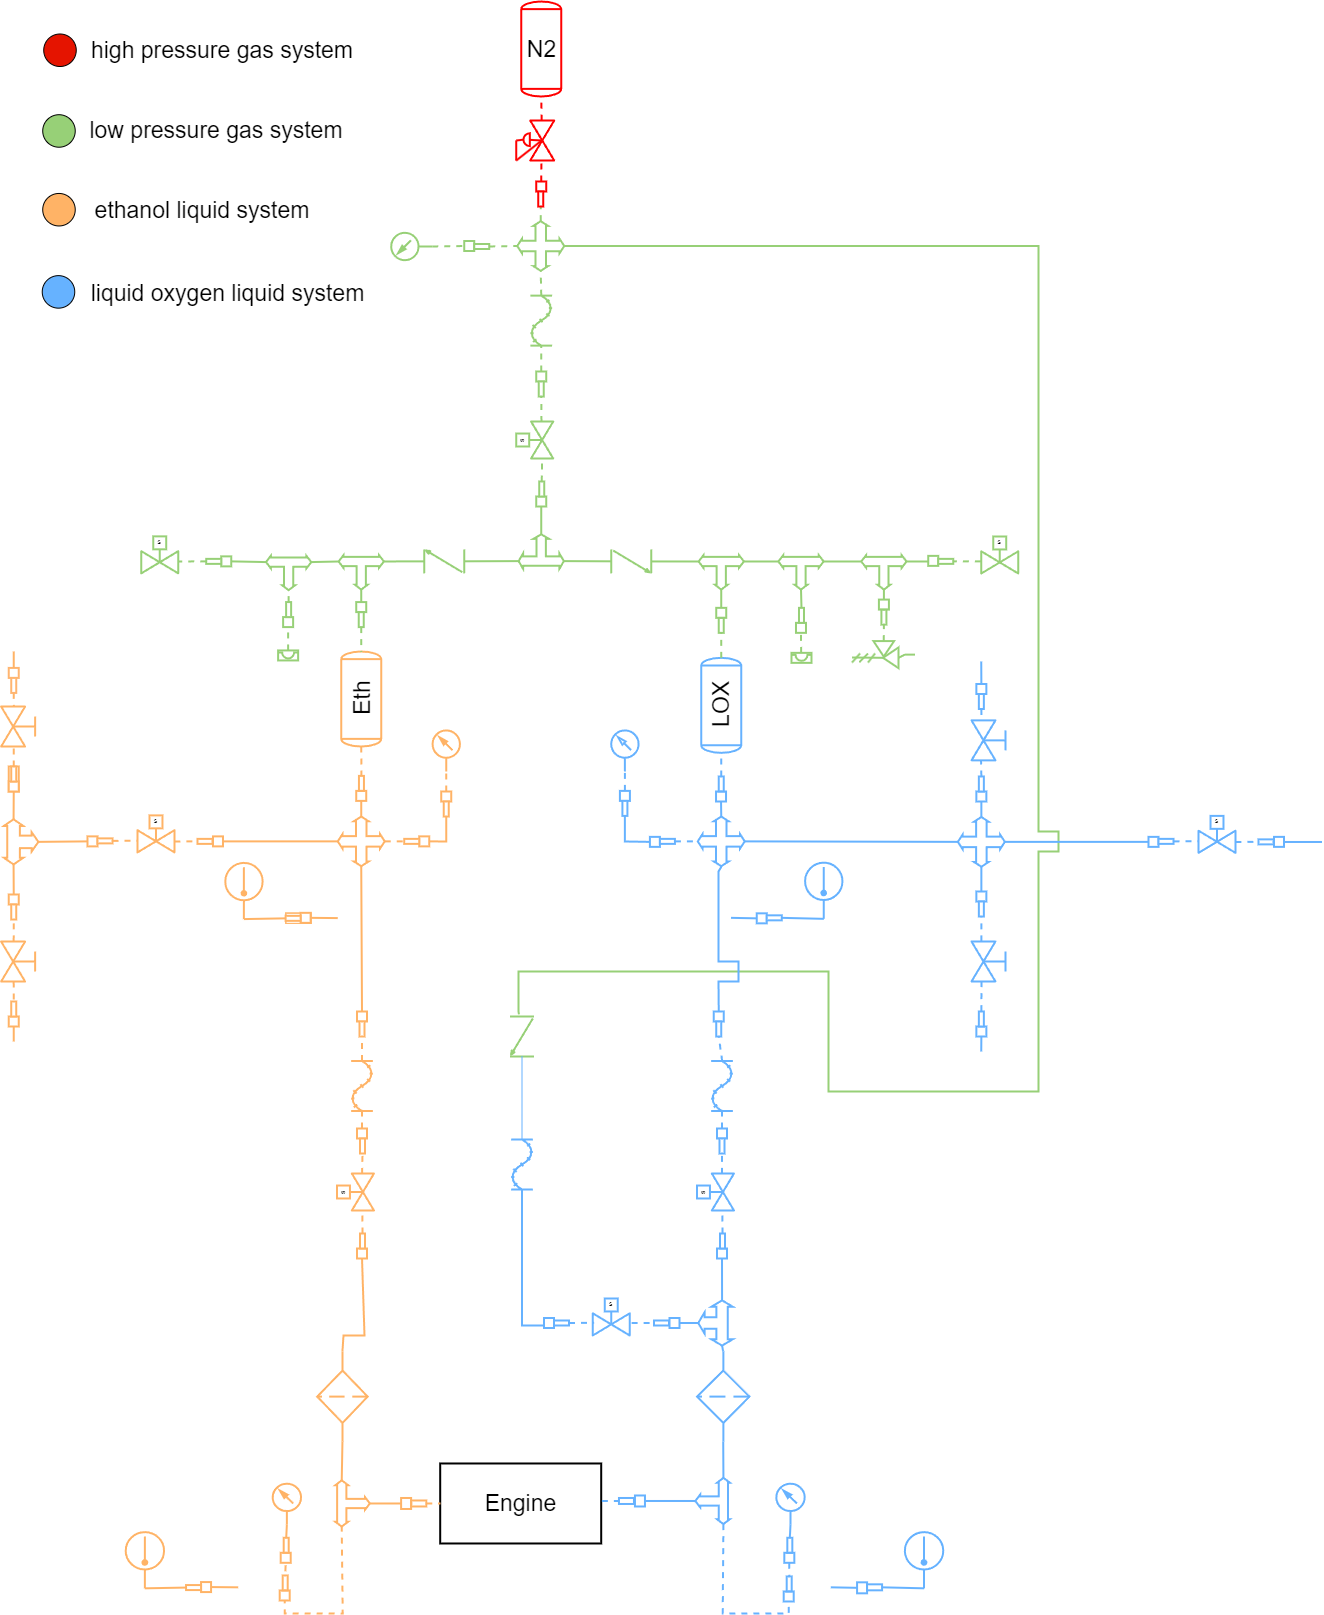
\includegraphics[width=1\linewidth]{figures/fluid_plan_4.1_simple.png}
                \caption{Sections of the simplified test stand fluid system}
                \label{fig:fluid_plan_sections}
            \end{figure}
            %
            \subsubsection{Plumbing}
            %
            \paragraph{Material}
                The materials of the tube system, and those of other components built in to it are determined not only by the pressure of the system, but also by their chemical resistance to the fluids used, their spontaneous ignition probability when in contact with pure gaseous and liquid oxygen at pressures above ambient and the burn resistance of the material once ignited. The material chosen for the tubing system is 316 stainless steel. This decision is based on a recommendation in the "NASA Glenn Safety Manual - Chapter 5 Oxygen". Here 316 Steel is one of the recommended metals for low pressure liquid oxygen service. In the manual, low pressure is defined as being below \qty{6.8948}{MPa} (\qty{1000}{psi}) of absolute pressure \cite[21]{glenn}. That all of the low pressure systems are below \qty{6.8948}{MPa} is validated in the section "Pressure" of this chapter. As the Swagelok tube system uses metal to metal seals, no sealant materials need be discussed for the tubing system. These will be addressed individually for each sub component below but will also draw on "NASA Glenn Safety Manual - Chapter 5 Oxygen" TABLE C.2.—SOME RECOMMENDED MATERIALS FOR OXYGEN SERVICE \cite[46]{glenn}. It must be remembered however, that under the right conditions, even stainless steel is flammable in high pressure oxygen environments. The NASA Glenn Safety Manual recommends keeping flow speeds of oxygen below \qty{30.48}{m/s} (\qty{100}{ft/s}) to avoid high speed entrainment of particulates. As their subsequent impact on a surface, such as a pipe bend, may deliver enough energy, to cause the steel to ignite \cite[25]{glenn}. The flow speeds achieved in the \qty{3}{kN} engine can be viewed in table \ref{tab:speed_of_flow}.
            %
            \paragraph{Tubing sizes}
                While both the diameter of the tubes and the system back pressure are determined by the required mass flow rate of the engine. A larger tube diameter makes the tubes heavier, bulkier and more difficult to bend and work with. It also gives the system a larger thermal mass, requiring more pre-chilling. On the other hand, a small tube diameter comes with a heavier loss in pressure and higher flow velocities at the same mass flow rate. The former necessitates a higher backing pressure at the same flow rate. The latter will result in higher pipe wall reaction forces in bends, increased fluid hammer on valve actuation and may increase the risk of spontaneous ignition in oxygen rich environments. In the end this decision was mainly driven by, availability of tube sizes and fittings for those sizes, ease of assembly and  precedence in other systems \cite[120]{mojave_sphinx}. The swagelok fitting system was chosen due to recommendation by ILR staff. The high pressure gas system does not use any tubing. The low pressure gas system uses tubes with an outer diameter of \qty{6.35}{mm} (\qty{0.25}{in}) and an inner diameter of \qty{4.572}{mm}. The low pressure gas system tubes are rated to a gauge pressure of \qty{35.1633}{MPa}. The low pressure liquid system tubes have an outer diameter of \qty{12.7}{mm} (\qty{0.5}{in}) and an inner diameter of \qty{9.398}{mm} and are rated at a gauge pressure of up to \qty{35.1633}{MPa} \cite[2]{SL_SS_Tubing}. An overview of the selected sizes for the 316 steel seamless tubing can be viewed in Table \ref{tab:tubesizes}. 
                %
                \begin{table}[h] 
                \centering
                    \begin{tabular}{ |p{3cm}| c | c| c|} 
                        \hline
                        Tube & Outer diameter in \qty{}{mm} & Inner diameter in \qty{}{mm} & Pressure rating in \qty{}{MPa} \\
                        \hline
                        High pressure  gas system & 6.35 & 4.572 & 35.1632\\
                        \hline
                        Low pressure gas system & 6.35 & 4.572 & 35.1632\\  
                        \hline
                        Low pressure liquid system & 12.7 & 9.398 & 35.16323\\
                        \hline
                    \end{tabular} 
                    \caption{Sizes and pressure ratings of tubing used in engine test stand.}
                    \label{tab:tubesizes}
                \end{table}
            %
            \paragraph{Pressure}
                \textbf{Note that pressure drop due to filters is TBD. It is not included as no filters have been selected. Furthermore, the effects of nitrogen dissolving into the LOX have not been accounted for jet.} The necessary pressure $p_1$ to apply with the inert gas to achieve the mass flow required can be estimated analytically using Bernoulli's equation with flow losses and energy inputs \ref{eq:bernoulli_flow_loss} \cite[118]{Paschereit:2022}.
                %
                \begin{align}
                    \frac{c_1^2}{2} + gz_1 + \frac{p_1}{\rho} +  \frac{\Delta p}{\rho} = \int_{1}^{2} \frac{\partial c}{\partial t} \, ds + \frac{c_2^2}{2} + gz_2 + \frac{p_2}{\rho} + \frac{\Delta p_L}{\rho} \label{eq:bernoulli_flow_loss}
                \end{align}
                %
                We will simplify equation \ref{eq:bernoulli_flow_loss} by assuming that both the engine and the fluid level in the tank are at equal heights. This eliminates the $gz$ terms. There is also no source of mechanical energy such as a pump, therefore the $\frac{\Delta p}{\rho}$ term turns to zero. Assuming the test stand is not in a transient state, the flow in the pipe can be considered fully steady, implying there is no time-dependent change in the vector field, therefore $\frac{\partial c}{\partial t} = 0$. Furthermore both entrance and exit pipe diameters shall be the same, assuming incompressibility, as before, the continuity equation, $c\cdot\rho\cdot A = const.$, dictates that flow speeds will be the same, eliminating the $\frac{c^2}{2}$ terms. All that remains is to rearrange for the back pressure $p_1$ which gives equation \ref{eq:backpressure}. Here $p_1$ is the system back pressure, $p_2$ is the engine chamber pressure and $\Delta p_L$ is the pressure loss term, resultant from energy dissipation over the system due to friction.
                 %
                \begin{align}
                    p_1 = p_2 + \Delta p_L\label{eq:backpressure}
                \end{align}
                %
                While $p_2$ is known, it is equal to the the sum of the thrust chamber pressure of the engine $p_c$ as seen in table \ref{tab:engine_parameters} and the minimum pressure drop over the injector, the pressure loss term $\Delta p_L$ is not. The pressure loss term must be calculated from pipe wall, fitting and valve friction. This can be done using equation \ref{eq:specific_pressure_loss} \cite[134]{Paschereit:2022}.
                  %
                \begin{align}
                    \frac{\Delta p_L}{\rho} = \text{Pipe wall friction} + \text{Fitting friction} + \text{Valve friction} \\
                    \frac{\Delta p_L}{\rho} = \sum_{\nu} \lambda_{\nu} \frac{L_{\nu}}{D_{\nu}} \frac{c_{\nu}^2}{2} + \sum_{\sigma} \zeta_{\sigma} \frac{c_{\sigma}^2}{2} + \frac{\Delta p_V}{\rho}\label{eq:specific_pressure_loss}
                \end{align}
                %
                First we shall focus on the calculation of the specific pressure loss due to pipe friction. The first summand in equation \ref{eq:specific_pressure_loss}. Here $\lambda$ is the unit less pipe friction factor, $L$ is the length of the pipe segment in \unit{m}, $c$ is the flow velocity in \unit{m/s}, $D$ is the inner Diameter of the pipe in \unit{m} and $\nu$ denotes the pipe segment.
                %
                The flow speeds $c$ of both media can be derived via the engine mass flows for oxygen and ethanol, which in turn are derived from the overall mass flow and the oxidizer-fuel fraction of the engine. The former is $\dot{m} = \qty{0.312}{kg/s}$ and the latter $\Phi_{Ox/Br} = 1.1$ which from now on will be refereed to as $\Phi_{O/Fu} = 1.1$ \cite[22]{mayer:2023}. Using the equation that defines the oxidizer-fuel-mass-fraction \ref{eq:oxedizer_fuel_mass_fraction} and the equation for the overall mass flow \ref{eq:massflow}, expressions for the ethanol \ref{eq:eth_mass_flow} and oxygen mass flow \ref{eq:oxygen_mass_flow} can be found. The reaction is to be cooled by diluting the ethanol with 20\% Water. The water fuel fraction is expressed by $\Phi_{H_2O/Fu}$ \ref{eq:massfraction_H2O_Fu} \cite[3]{mayer:2023}. Solving equation \ref{eq:massfraction_H2O_Fu} and \ref{eq:massfraction_Eht_Fu} for the fuel mass flow rate we receive equation \ref{eq:fuel_mass_flow}. Given no further margin this leaves the mass flow rates found in the second column of table \ref{tab:massflows} .
                %
                \begin{multicols}{2}
                    \begin{align} 
                        \dot{m} = \dot{m}_{Fu} + \dot{m}_{O} \label{eq:massflow}
                    \end{align}
                    \begin{align}
                        \Phi_{O/Fu} = \frac{\dot{m}_{O}}{\dot{m}_{Fu}} \label{eq:oxedizer_fuel_mass_fraction}
                    \end{align}
                \end{multicols}
                %
                \begin{multicols}{2}
                    \begin{equation}
                        \dot{m}_{Eth} = \frac{\dot{m}}{\Phi_{O/Fu} + 1} \label{eq:eth_mass_flow}
                    \end{equation}
                    \begin{equation}
                        \dot{m}_O = \frac{\dot{m}\cdot \Phi_{O/Fu}}{1 + \Phi_{O/Fu}} \label{eq:oxygen_mass_flow} 
                    \end{equation}
                \end{multicols}
                %
                \begin{equation}
                    \dot{m}_{Fu} = \frac{\dot{m}_{Eth}}{1 - \Phi_{H_2O}} \label{eq:fuel_mass_flow}
                \end{equation}
                %
                The upper bound of engine to be tested on the stand shall be of a force of \qty{3}{kN}. The mass flow rates necessary for such an engine can be estimated using the current engines specific impulse of $I_{sp} = \qty{2418.7}{m/s}$. While the $I_{sp}$ of future engines will probably be lower due to the systems maximum pressure rating, with an appropriate margin, this provides a rough design point to base the test stands fluid system design on. Equation \ref{eq:massflow_from_force} can be used to find out the overall mass flow, then using the equations \ref{eq:eth_mass_flow} and \ref{eq:oxygen_mass_flow} individual mass flows are determined. Results can be found in column three of table \ref{tab:massflows}.
                %
                \begin{align}
                    \dot{m} = \frac{F}{I_{sp}} \label{eq:massflow_from_force}
                \end{align}
                %
                \begin{table}[h]
                \centering
                    \begin{tabular}{ |l | c | c|} 
                        \hline
                        Component & Mass flow in \qty{}{kg/s} (\qty{750}{N}) & Mass flow in \qty{}{kg/s} (\qty{3}{kN}) \\
                        \hline
                        Combined & 0.3101 & 1.2403\\
                        \hline
                        Oxidizer & 0.1624 & 0.6497\\  
                        \hline
                        Fuel & 0.1846 & 0.7383 \\
                        \hline
                    \end{tabular} 
                    \caption{Engine mass flow rates used as design points for engine test stand fluid system development.}
                    \label{tab:massflows}
                \end{table}
                %
                Using the mass flows we previously found, we can now estimate the flow velocities of both the ethanol water fuel mix and the liquid oxygen. Equation \ref{eq:flowspeed} shows how the mass flow $\dot{m}$, the density of the fluid $\rho$, the permeated area $A$ and the flow velocity $c$ are related. The permeated area in our case being the inner cross section of the pipe. This can be calculated using equation \ref{eq:A_circle}.
                %
                \begin{multicols}{2}
                    \begin{equation}
                        c = \frac{\dot{m}}{\rho A} \label{eq:flowspeed}
                    \end{equation}
                    \begin{equation}
                        A = \pi\left(\frac{D}{2}\right)^2 \label{eq:A_circle}
                    \end{equation}
                \end{multicols}
                %
                Of curs calculation of the flow speed via equation \ref{eq:flowspeed} requires that we know the densities of our fluids. Therefore the ambient temperature was set to be \qty{288.15}{K}, as was the ethanol temperature. The initial temperature of the liquid oxygen will be its ambient pressure boiling temperature of \qty{90.19}{K}, assuming the oxygen is supplied from a dewar. A dewar is a none pressurized cryogenic container that continuously vents boil off gas to maintain its temperature used for storing small amounts of cryogenics up to \qty{200}{l}. While the ethanol water mix will remain at ambient temperature throughout the test, changes in the temperature of the liquid oxygen are to be expected, as it is heated through the tank walls. This change in temperature will impact the density of the liquid, and thereby the flow speed necessary to supply the needed mass flow. To illustrate this fact, flow speeds for the densest and least dense expected configurations where calculated. In the first configuration, saturated liquid oxygen is filled in to the propellant tanks at ambient pressure. Then it is pressurized, using the Nitrogen gas system, to a pressure of about \qty{4}{MPa}. While this pressure is merely a guess at the moment, the low compressibility of the liquids, makes the change in density of the liquids in response to pressure change quite low. The situation is idealized and no conductive heating of the liquid oxygen occurs. It remains at its ambient pressure saturation temperature of \qty{90.19}{K}. This would be the chase if the engine was fired shortly after pressurization. The second configuration extends the first, by allowing the pressurized liquid oxygen to heat up to its boiling temperature at $p_1$, the system back pressure. The liquid begins to boil and and increase tank pressure until the set pressure of the relief valve at \qty{4}{MPa} is reached. From here on the liquid phases temperature and density remain the same, continuously cooled by evaporation. The liquid oxygen has reached its highest temperature of \qty{145.3645}{K} and thereby lowest density. Compression heating will be neglected for both chases, as its impacts lay in the sub \qty{1}{K} range. The resulting densities used for the calculations can be found in table \ref{tab:densities}. All material properties listed where found with the help of CoolProp.jl. This is a Julia wrapper for the CoolProp open-source thermophysical property library written in C\texttt{++} \cite{coolprop_article}.
                %
                \begin{table}[h] 
                \centering
                    \begin{tabular}{ |l | c | c|} 
                        \hline
                        Fluid  & Density in \unit{kg/m^3} & Temperature in \unit{K}\\
                        \hline
                        Oxidizer config. 1 & 1148.5768 & 90.1878\\
                        \hline
                        Oxidizer config. 2 & 700.3576  & 148.6593\\  
                        \hline
                        Fuel & 837.3932 & 288.15\\
                        \hline
                    \end{tabular} 
                    \caption{Density and temperature of fuel, oxidizer at ambient saturation temperature at \qty{4}{MPa} (config. 1) and saturated oxidizer (config. 2) at \qty{4}{MPa} of pressure.}
                    \label{tab:densities}
                \end{table}
                %
                Using the densities in table \ref{tab:densities} and equation \ref{eq:flowspeed} the required flow speeds where calculated for both the \qty{750}{N} and the \qty{3}{kN} engine. The results can be viewed in table \ref{tab:speed_of_flow}. The large difference in flow speed between the two oxidizer configurations of \qty{60.92}{\%} is of great importance. Neither the system back pressure nor the system geometry may be varied during the test. As a result, the mass flow rate of the oxidizer will vary depending on the liquid oxygen's temperature, which in turn calls for tank temperature measuring capabilities, which will be discussed further in a later chapter. This means the system needs to be designed for a specific LOX temperature. Due to the higher flow speeds necessary, which increases spontaneous combustion probability, the possibility of gas bubbles entering the injector, which increase combustion instability and president from literature \cite[203]{Sutton:2021} it was decided to fire the engine shortly after pressurization, when the liquid oxygen is still at its ambient pressure boiling temperature of \qty{90.19}{K} (config. 1). 
                %
                \begin{table}[h]
                \centering
                    \begin{tabular}{ |l | c | c|} 
                        \hline
                        Fluid  & Speed of flow in \unit{m/s} (\qty{750}{N}) & Speed of flow in \unit{m/s} (\qty{3}{kN})\\
                        \hline
                        Oxidizer config. 1 & 2.0386 & 8.1544\\
                        \hline
                        Oxidizer config. 2 & 3.3639 & 13.3731\\  
                        \hline
                        Fuel & 3.1775 & 10.1632\\
                        \hline
                    \end{tabular} 
                    \caption{Flow speed of fuel at \qty{288.15}{K}, oxidizer at ambient saturation temperature \qty{90.19}{K} (config. 1) and oxidizer at \qty{4}{MPa} saturation temperature \qty{145.3645}{K} (config. 2), in \qty{9.398}{mm} diameter pipe at \qty{4}{MPa} of pressure.}
                    \label{tab:speed_of_flow}
                \end{table}
                
                Returning to equation \ref{eq:specific_pressure_loss}, the means of calculation for the pipe friction factor $\lambda$ varies depending on if the flow is laminar or turbulent. This in turn is characterized by the Reynolds-number. In a pipe, flow is judged to be fully turbulent above a Reynolds-number of \num{5000} \cite[120]{Paschereit:2022}. The Reynolds-number for a circular pipe is calculated using equation \ref{eq:reynolds_pipe} \cite[629]{Paschereit:2022}.
                %
                 \begin{multicols}{2}
                    \begin{equation}
                        Re = \frac{cD}{\nu}  \label{eq:reynolds_pipe} 
                    \end{equation}
                    \begin{equation}
                        \eta_{\text{lmix}} = \exp\left(\sum_{i=1}^{N} x_{i} \ln( \eta_{li})\right)  \label{eq:Grunberg-Nissan}
                    \end{equation}
                \end{multicols}
                %
                In equation \ref{eq:reynolds_pipe} the dynamic viscosity's $\eta$ and densities $\rho$ for water and ethanol at \qty{4}{MPa}, \qty{288.15}{K} and LOX at \qty{4}{MPa}, \qty{90.19}{K} used for calculating the kinematic viscosity $\nu$ where found using CoolProp \cite{coolprop_article}. Using the Grunberg-Nissan equation \ref{eq:Grunberg-Nissan} \cite{Grunberg-Nissan}, the dynamic viscosity of the fuel mixture, consisting of \qty{20}{\%} Water and \qty{80}{\%} Ethanol, was calculated. In the Grunberg-Nissan equation $\eta_{li}$ are the dynamic viscosities of the individual pure liquids that make up the mixture. $x_i$ are the mole fractions of the mixture components, these where calculated using equation \ref{eq:molefractions}. 
                %
                \begin{multicols}{2}
                    \begin{equation}
                        \Phi_{H_2O/Fu} = \frac{m_{H_2O}}{m_{H_2O}+ m_{Eth}}  \label{eq:massfraction_H2O_Fu} = 0.2
                    \end{equation}
                    \begin{equation}
                        \Phi_{Eth/Fu} = \frac{m_{Eth}}{m_{H_2O}+ m_{Eth}}  \label{eq:massfraction_Eht_Fu} = 0.8
                    \end{equation}
                    \begin{equation}
                        b_i = \frac{\Phi_{i/Fu}}{M_i} \label{eq:molalitys}
                    \end{equation}
                    \begin{equation}
                        x_i = \frac{b_{Eth} + b_{H_2O}}{b_i}  \label{eq:molefractions}
                    \end{equation}
                \end{multicols}
                %
                In equation \ref{eq:molefractions} the numerator is the sum of the molality of both ethanol and water, which is equal to the inverse molar mass of the mixture. The denominator is the molality of the substance who's mole fraction is to be calculated. The molality of each substance can be calculated using equation \ref{eq:molalitys}. Here $M_i$ is the molar mass of the substance in question, found using coolprop \cite{coolprop_article} and $\Phi_{i/Fu}$ is the mass fraction of either water or ethanol in the fuel mixture as defined by equations \ref{eq:massfraction_H2O_Fu} and \ref{eq:massfraction_Eht_Fu}.
                
                Having found the dynamic viscosity $\eta$ of both the fuel and the oxidizer, the kinematic viscosity $\nu$ which is required for the Reynolds-number can be found using equation \ref{eq:kinematic_viscosity} \cite[24]{Paschereit:2022}. Here the densities $\rho$ where taken form table \ref{tab:densities}. 
                %
                \begin{equation}
                    \nu = \frac{\eta}{\rho}  \label{eq:kinematic_viscosity}
                \end{equation}
                %
                Using the inner diameter of the low pressure piping given in table \ref{tab:tubesizes}, the calculated flow velocities from table \ref{tab:speed_of_flow} and the kinematic viscosity's just found, the Reynolds-numbers where calculated. The results are listed in table \ref{tab:Reee}.
                %
                \begin{table}[H]
                \centering
                    \begin{tabular}{ |l | c | c|}
                        \hline
                        Fluid  & Re-number (750\unit{N}) & Re-number (3\unit{kN})\\
                        \hline
                        Oxidizer config. 1 & 109272.1635 & 437088.6542 \\
                        \hline
                        Fuel & 19839.3684 & 79357.4736\\
                        \hline
                    \end{tabular} 
                    \caption{The Reynolds-numbers of the flow of fuel at \qty{288.15}{K} and oxidizer at \qty{90.19}{K} (config. 1).}
                    \label{tab:Reee}
                \end{table}
                %
                From table \ref{tab:Reee} one can tell, that none of the Reynolds-numbers lay below 5000. This means the pipe flow is fully turbulent and the Colebrook-White-Equation \ref{eq:pipe_friction_factor} can be used to calculate the pipe friction factor \cite[121]{Paschereit:2022}.
                %
                \begin{equation}
                        \frac{1}{\sqrt{\lambda}} = -2.0 \log_{10} \left( \frac{2.51}{\text{Re} \sqrt{\lambda}} + \frac{0.27 \epsilon}{D} \right)  \label{eq:pipe_friction_factor}
                \end{equation}
                %
                As the equation is non-linear and implicit the Julia Roots.jl package \cite{Roots.jl} was employed to solve the equation using iteration. The inner pipe roughness $\epsilon$ for the low pressure piping is \qty{1.6256}{\mu m} \cite{mail}. With all necessary inputs successfully procured, the pressure loss due to pipe wall friction was calculated by rearranging the first summand of equation \ref{eq:specific_pressure_loss} to equation \ref{eq:pipe_friction_pressure_drop}.
                %
                \begin{align}
                    \Delta p = \lambda \frac{L}{D} \frac{c^2}{2}
                    \label{eq:pipe_friction_pressure_drop}
                \end{align}
                %
                Here a pipe length $L$ of \qty{3}{m} was assumed. The results can be found in table \ref{tab:pipe_friction_pressure_drop}.\\
                %
                \begin{table}[H]
                \centering
                    \begin{tabular}{ |l | c | c|}
                        \hline
                        Fluid  & Pressure drop in \unit{kPa} (750\unit{N}) & Pressure drop in \unit{kPa} (3\unit{kN})\\
                        \hline
                        Oxidizer config. 1 & 14.1628 & 187.5026\\
                        \hline
                        Fuel & 35.5007 & 424.6853\\
                        \hline
                    \end{tabular} 
                    \caption{Pressure drop due to pipe friction of  fuel at \qty{288.15}{K} and oxidizer at \qty{90.19}{K} (config. 1).}
                    \label{tab:pipe_friction_pressure_drop}
                \end{table}
                %
                For the calculation of the pressure drop due to fixtures, namely bends in the pipe system, the pressure loss number $\xi$ must be found. With a bend radius to pipe diameter ratio of $R/D = 4$ we receive a pipe radius of \qty{50.8}{mm} and a pressure loss number of $\zeta = \num{0.15}$. Using this number, the flow speeds from table \ref{tab:speed_of_flow} and assuming 3 equal bends the pressure drop can be calculated by rearranging the second summand of equation \ref{eq:specific_pressure_loss} into \ref{eq:pipe_fixture_pressure_drop}. The results of this calculation can be seen in table \ref{tab:pipe_fixture_pressure_drop}.
                %
                \begin{align}
                    \Delta p = 3 \cdot \rho  \cdot\zeta \frac{c^2}{2}
                    \label{eq:pipe_fixture_pressure_drop}
                \end{align}
                %
                \begin{table}[H]
                \centering
                    \begin{tabular}{ |l | c | c|}
                        \hline
                        Fluid  & Pressure drop in \unit{kPa} (750\unit{N}) & Pressure drop in \unit{kPa} (3\unit{kN})\\
                        \hline
                        Oxidizer config. 1 & 1.0740 & 17.1841 \\ 
                        \hline
                        Fuel & 1.9023 & 30.4363 \\
                        \hline
                    \end{tabular} 
                    \caption{Pressure drop due to fixtures of  of  fuel at \qty{288.15}{K} and oxidizer at \qty{90.19}{K} (config. 1).}
                    \label{tab:pipe_fixture_pressure_drop}
                \end{table}
                %
                In addtiton the pressure loss due to the installed valves must be calculated. This can be derived from the valves flow coefficient $K_V$. For both the liquid oxygen main valve KB-20-NC (Appendix \ref{appendix:KB_20_NC_2E}) and the fuel main valve MK-15-NC-2E (Appendix \ref{appendix:MK_15_NC_2E}) this factor is $K_V = 2.5$. Rearranging the definition of the flow coefficient \cite[34]{Zappe:2004} in equation \ref{eq:Flow_coefficient} the pressure drop can be calculated using equation \ref{eq:valve_pressure_drop}.
                %
                \begin{multicols}{2}
                    \begin{equation}
                        K_V = \dot{V} \sqrt{\frac{\qty{1}{bar}}{\Delta p} \cdot \frac{\rho}{\qty{1000}{\frac{kg}{m^3
                        }}}}  \label{eq:Flow_coefficient}
                    \end{equation}
                    \begin{equation}
                        \Delta p = \qty{1}{bar} \cdot \frac{\rho}{\qty{1000}{kg}} \left( \frac{\dot{V}}{{K_V}} \right)^{2} \label{eq:valve_pressure_drop}
                    \end{equation}
                \end{multicols}
                %
                The volume flows $\dot{V}$ where calculated using equation \ref{eq:volumeflow}. The mass flows $\dot{m}$ used can be found in table \ref{tab:massflows}, the fluid density's $\rho$ are taken from table \ref{tab:densities}. The pressure drops received by evaluation of equation \ref{eq:valve_pressure_drop} can be found in table \ref{tab:valve_pressure_drop}.
                %
                \begin{equation}
                    \dot{V} = \frac{\dot{m}}{\rho} \label{eq:volumeflow}
                \end{equation}
                %
                \begin{table}[H]
                \centering
                    \begin{tabular}{ |l | c | c|}
                        \hline
                        Fluid  & Pressure drop in \unit{kPa} (750\unit{N}) & Pressure drop in \unit{kPa} (3\unit{kN})\\
                        \hline
                        Oxidizer config. 1 & 4.7629 & 76.2062\\ 
                        \hline
                        Fuel & 8.4360 & 134.9757\\
                        \hline
                    \end{tabular} 
                    \caption{Pressure drop due to valve friction of of  fuel at \qty{288.15}{K} and oxidizer at \qty{90.19}{K} (config. 1).}
                    \label{tab:valve_pressure_drop}
                \end{table}
                %
                The sum of all of these pressure drops can be read from table \ref{tab:overall_pressure_drop}.
                %
                \begin{table}[H]
                \centering
                    \begin{tabular}{ |l | c | c|}
                        \hline
                        Fluid  & Pressure drop in \unit{kPa} (750\unit{N}) & Pressure drop in \unit{Bar} (3\unit{kN})\\
                        \hline
                        Oxidizer config. 1 & 0.2000 & 2.8090\\
                        \hline
                        Fuel & 0.4584 & 5.901\\
                        \hline
                    \end{tabular} 
                    \caption{Over all pressure drop in the low pressure fluid system of  fuel at \qty{288.15}{K} and oxidizer at \qty{90.19}{K} (config. 1).}
                    \label{tab:overall_pressure_drop}
                \end{table}
                %
                To illustrate the systems pressure loss response to any mass flow a system characteristic curve \ref{fig:system_characteristic curve} of the test stand can be found below. This was achieved by performing the above calculations on an array of mass flows. These where gained by dividing an array of engine thrusts by the \qty{750}{N} engines Isp yielding the mass flow rate of any engine of equal Isp using the same propellants.
                %
                \begin{figure}[h]
                    \centering
                    \includesvg[width=1\linewidth]{figures/System_curve.svg}
                    \caption{Fluid system characteristic curve of pressure drop in \unit{bar} over mass flow in \unit{kg/s} and thrust in \unit{kN}.}
                    \label{fig:system_characteristic curve}
                \end{figure}
                
        \subsubsection{High Pressure Gas System}
        %
        \subsubsection{Low Pressure Gas System}
 
        %
        \subsubsection{Low Pressure Liquid System}
        %
        \subsubsection{Validation}


    \subsection{Physical Structure}
        \subsubsection{Requirements and Constraints}

    \subsection{Tank Design}
        \subsubsection{Requirements and Constraints}
The ethanol and LOX tank must each hold approx. 20 liters, have a burst pressure of 100 bar and be as affordable and easy to manufacture as possible. The LOX tank must also be able to withstand the cryogenic temperatures of LOX at an operating pressure of approximately 40 bar. Temperatures of 158 K are expected. Furthermore, the LOX tank is insulated to prevent the LOX from boiling.\\
All pressure vessels must be inspected by the TÜV before use. 
\subsubsection{Volume}
The tanks are made from round pipes with an internal diameter of 132.7 mm and a height of 150 cm. For the lids, 2 cm per side are not included in the height of the volume calculation. Thus: $h_{tank} = 1,46 m$; $d_{tank_{in}} = 0,1327 m$\\
$$Volume_{tank,in} = \left(\frac{d_{tank,in}}{2}\right)^2 \cdot \pi \cdot h_{tank,in} = 0.22 \, \text{m}^3$$ \\ 

LOX is highly reactive. To avoid corrosion, the LOX tank is made of stainless steel. An S235JR with the same diameter and height has already been purchased and can be used for the ethanol tank. If the budget allows, a second stainless steel pipe should be used.
\newline
\begin{tabular}{ll}
    ${h}_{tank,in}$:    & hight of the inner tankwall \\
    ${d}_{tank,in}$:    & inner diamiter of the tank \\
    ${V}_{tank,in}$:    & inner volum of the tank \\
\end{tabular}
\newline
\subsubsection{Wall thickness and Pressure calculation}
The wall thickness is determined using the Barlow's formula under the following assumptions:
\begin{enumerate}
    \item \qty{100}{Bar} burst pressure
    \item \qty{360}{MPa} Tensile strength
    \item \qty{0.13}{m} medium diameter
\end{enumerate}
Leads to:\\
$s_{tangential} = \frac{P\cdot d_m}{2\cdot\sigma}=1.8917mm;$\\
$s_{axial} = \frac{P\cdot d_m}{4\cdot\sigma}=0.9458mm$\\
The selected pipe has a wall thickness of \textbf{4mm} and thus offers additional safety. Consultations with the design department revealed that lids of the same thickness can be welded particularly well. For this reason, 4 mm thick plates were also chosen for the lids.
\newline
\begin{tabular}{ll}
    ${s}_{tangential}$: & allowable stress tangential \\
    ${s}_{axial}$:      & allowable stress axial \\
\end{tabular}
\newline
\subsection{Tank Weldment calculation}
To calculate the strength of a weldment the applied Force perpendicular to the weld has to be determined. This is done by first calculating the area of the attack on which the force is applying its load.
\begin{gather}
    A = \left( \frac{d_{tank,in}}{2} \right)^2 \cdot \pi = 0,0138 \hspace{1ex} \text{mm}^2
\end{gather}
Thus now the force exerted can be calculated:
\begin{gather}
    F_z = A \cdot P = 138303,04 \hspace{1ex} \text{N}
\end{gather}
For further calculation an assumpsion of the weld thickness is needed. For wall thicknesses of $\geq 4 \text{mm}$ a weld thickness of atleast $a = 3 \text{mm}$ is to be assumed \cite[Eq. 6.17a, P. 176]{roloff}. Additionaly the outer diamater of the pipe is determined as $d_{out} = 136,7 \text{mm}$
With this it is now possible to calculate the perpendicular stress in the weld $\sigma_{90}$ \cite[Pic. 6.46, P. 186]{roloff}:
\begin{gather}
    \sigma_{90} = \frac{F_z}{a \cdot \pi \cdot d_{out}} = 107,35 \hspace{1ex} \frac{\text{N}}{\text{mm}^2}
\end{gather}
Which according to \cite[Eq. 6.19, P. 179]{roloff} has to satisfy following equation, where $R_m = 360 \frac{\text{N}}{\text{mm}^2}$ and parts safty value $\gamma_{M2} = 1,25$:
\begin{gather}
    \sigma_{90} = 107,35 \hspace{1ex} \frac{\text{N}}{\text{mm}^2} \leq 259,2 \frac{\text{N}}{\text{mm}^2} = 0,9 \cdot \frac{R_m}{\gamma_{M2}}
\end{gather}
To calculate the maximum pressure (vertical force acting on the lid weldment) the maximum allowed stress in this weldment has to be determined. According to the weld situation "77" that has been choosen the worst case is an allowed $\sigma_{max} = 105 \frac{\text{N}}{\text{mm}^2}$ with the "Notch-Integrity-Line" being F2\cite[Tab. 6-11, 6-12]{roloff}. With this the maximum force till failure (with extra safty) can be calculated:
\begin{gather}
    F_{max} = \sigma_{max} \cdot a \cdot \pi \cdot d_{tank,out} = 135278,55 \hspace{1ex} \text{N}
\end{gather}
Or even further the theoretical pressure can be calculated:
\begin{gather}
    P_{max} = \frac{F_{max}}{A} = 97,813 \hspace{1ex} \text{bar}
\end{gather}
Thus the weld structure has been verified.\\
\begin{tabular}{ll}
    $A$:                & area on which load is applied (lid) \\
    ${F}_{z}$:    & pressure force on lid \\
    ${a}$:    & weld thickness \\
    ${d}_{tank,in}$:    & inner diameter of the tank \\
    ${d}_{tank,out}$:    & outer diameter of the tank \\
    ${\sigma}_{90}$:    & perpendicular stress \\
    ${R}_{m}$:    & tensile strength \\
    ${\gamma}_{M2}$:    & parts safety value \\
    ${\sigma}_{max}$:    & worst case maximum allowed stress\\
    ${F}_{max}$:    & maximal force\\
    ${P}_{max}$:    & maximal pressure\\
\end{tabular}

    \subsubsection{LOX Tank Isolation}
The isolation thickness of the tanks depends on the required vaporization rate of the LOX. The vaporization rate is calculated:
\begin{gather} \label{eq:vaporization}
    \dot{m}_{LOX,vap} = \Delta h_v \cdot \dot{Q}_{tank}
\end{gather}
where
\newline
\begin{tabular}{ll}
    $\dot{m}_{LOX,vap}$: & mass flow of vaporized LOX \\
    $\Delta h_v$:        & enthalpy of vaporization \\
    $\dot{Q}_{tank}$:    & heat transfer rate through tank walls \\
\end{tabular}
\newline
The heat transfer between the air surrounding the tank and the LOX consists of convection between the fluids and the tank and conduction from the inside of the tank to the outside of the tank, as seen in figure \ref{fig:heat transfer}. \cite[33-34]{wärmeatlas}
\begin{figure}[h]
    \centering
    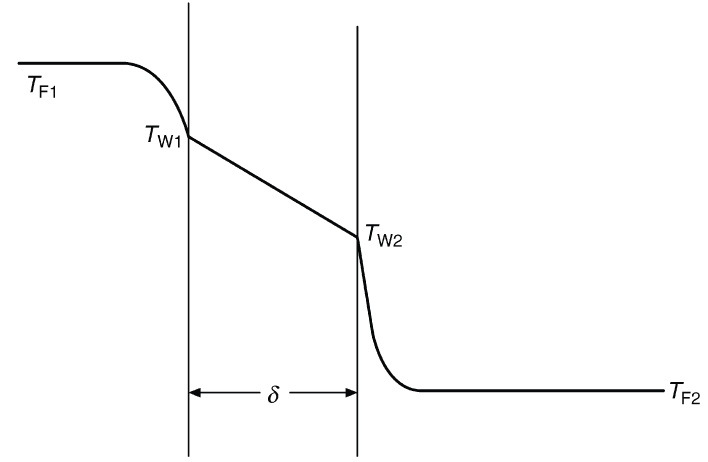
\includegraphics[width=0.5\linewidth]{figures/heat transfer.png}
    \caption{Heat transfer between two fluids separated by a wall \cite[33]{wärmeatlas}}
    \label{fig:heat transfer}
\end{figure}
The conduction can be calculated according to \cite[23]{wärmeatlas}:
\begin{gather}
    \dot{Q}_{tank} = k_{tank} \cdot A_{tank} \cdot \frac{T_{W1} - T_{W2}}{d_{tank}}
\end{gather}
where
\newline
\begin{tabular}{ll}
    $k_{tank}$: & thermal conductivity of the tank \\
    $T_{W1}$:   & temperature of the outer tank wall \\
    $T_{W2}$:   & temperature of the inner tank wall \\
\end{tabular}
\newline
The convection can be calculated according to \cite[757-758]{wärmeatlas}:
\begin{gather}
    \dot{Q}_{tank} = \alpha \cdot A_{tank} \cdot (T_{W} - T_{F})
\end{gather}
$\alpha$ is the heat transfer coefficient that describes the heat transfer between a fluid and a solid. For a cylinder it can be approximated according to \cite[759-760]{wärmeatlas}:
\begin{gather}
    \alpha = \frac{k_{tank}}{L_{char}} (0.752 + 0.387 \ (Pr \cdot Gr \ (1 + \left(\frac{0.559}{Pr}\right)^{\frac{9}{16}})^{\frac{-16}{9}})^{\frac{1}{6}})^2
\end{gather}
where
\newline
\begin{tabular}{ll}
    $L_{char}$: & characteristic length \\
    $Pr$:       & Prandtl number \\
    $Gr$:       & Grashof number \\
\end{tabular}
\begin{gather}
    L_{char} = \frac{\pi}{2} \cdot d_{tank}
\end{gather}
\begin{gather}
    Gr = \frac{g \cdot \beta \cdot (T_W - T_F) \cdot L_{char}^3}{\nu^2}
\end{gather}
$\beta$ is the coefficient of volume expansion and equal to approximately 1/T for ideal gases.
\newline
The boiling temperature of the LOX and the temperature of the air in the environment are known. The inside wall temperature can be assumed to be the same as the temperature of the LOX. However, the outside wall temperature is still needed to calculate the heat transfer rate. As there are too many unknowns there is no analytical way to determine the heat transfer rate. Thus a numerical approach is used to approximate $\dot{Q}_{tank}$.
\newline
First a outside wall temperature is assumed. With this assumed temperature a $\dot{Q}_{tank}$ is calculated. With this calculated $\dot{Q}_{tank}$ and the assumed outside wall temperature an inside wall temperature is calculated. The difference between this calculated inside wall temperature and the assumed inside wall temperature, which is the temperature of the LOX, is subtracted from the assumed outside wall temperature. The calculation are done again until the calculated inside wall temperature is within a tolerance of the assumed inside wall temperature.
\newline
For the isolation material the \textit{Froth-Pak Foam System} with a thermal conductivity $k_{iso}$ of 0.022 $ \frac{W}{m \cdot K}$ \ref{appendix:Fomicon}is chosen. With a tank pressure of 46 bar and an isolation thickness of 4 cm the heat transfer rate $\dot{Q}_{tank}$ is approximately 73.38 W. The enthalpy of vaporization $\Delta h_v$ for LOX at this pressure is 61.37 $\frac{kJ}{kg}$. Using equation \ref{eq:vaporization} results in a mass flow $\dot{m}_{LOX,vap}$ of 1.2 $\frac{g}{s}$.

\subsection{Electronic System}
This proposal outlines the development of a test stand electronics system for the BEARS propulsion group, designed to integrate a rocket engine with a thrust capacity of approximately 750 newtons, fueled by ethanol and liquid oxygen (LOX). The preferred implementation utilizes National Instruments (NI) hardware and LabVIEW software to facilitate testing and data acquisition. 
        
\subsubsection{Requirements and Constraints}

The following requirements are proposed for the test stand electrical system:

\textbf{Fluid System Control}
    \begin{itemize}
        \item The electronics system shall individually distribute and switch power to each valve in the fluid system.
        \item The electronics system shall regulate and maintain electrical power quality within the rated specifications of the fluid system valves.
        \item The electronics system shall respond to operator commands and change valve states within 50ms.
        \item The electronics system shall automatically switch the valves to a predefine semi-safe state if out-of-range conditions are detected.
        \item The electronics system shall respond to a physical emergency-stop at the operator station in order to put the fluid system into a predefined semi-safe state. See "Test Operator Interface" requirements
        \item The electronics system shall have a fault-tolerant architecture such that a single failure does not allow for an unsafe engine state.
    \end{itemize}

\textbf{Sensor Data}
    \begin{itemize}
        \item The electronics system shall include sensors to measure fluid line pressure near the propellant sources and near the engine, as well as at the propellant-feed source.
        \item The electronics system shall include sensors to measure fluid line temperature near the propellant sources and near the engine.
        \item The electronics system shall include sensors that can be used to measure or determine the mass-flow rates of the propellant.
        \item The electronics system shall include a sensor to measure or determine the thrust of the engine.
        \item All sensors in the electronics system shall be rated beyond the expected temperature, pressure, and mechanical load ranges of the locations in which they are installed.
        \item The electronics system shall take measurements at the required sample rates as specified by the fluid system requirements.
        \item The electronics system shall store measurement values until they have been sent to the operator station.
        \item The electronics system shall distribute electrical power to all active sensors.
        \item The electronics system shall regulate and maintain power quality within the rated specifications of the active sensors.
    \end{itemize}

\textbf{Test Operator Interface}
    \begin{itemize}
        \item The electronics system shall include a physical emergency-stop within reach of the test operator. See "Fluid System Control Requirements"
        \item The electronics system shall send sensor data to the operator station at a rate of at least 10Hz.
        \item The electronics system shall receive commands from the operator station within 10ms of them being sent.
        \item The electronics system shall provide a graphical user interface for the test operator, which displays sensor data and provides a method of sending commands.
        \item The test operator interface shall have a fault-tolerant architecture such that a single failure in the interface does not prevent the operator from viewing sensor data.
    \end{itemize}


\subsubsection{LabVIEW Proposal}

    \textbf{Measurement Inputs}
    
    To effectively monitor the test stand, the following sensors and modules are proposed:
    
    \begin{itemize}
        \item \textbf{Pressure Sensors:}
        \begin{itemize}
            \item 5 x Althen 4003 Pressure Transducers (4-20 mA output) for measuring LOX, ethanol, and Nitrogen feed line pressures, as well as ethanol and LOX engine pressures.
        \end{itemize}
        \item \textbf{Temperature Sensors:}
        \begin{itemize}
            \item 4 x PT-100 RTD Sensors with corresponding measurement transducers, interfaced via an NI-9217 RTD Analog Input Module. These measure ethanol and LOX temperatures near the tanks and near the engine.
        \end{itemize}
    % I thought we decided we would only use the tank weights for mass flow calculations
    %    \item \textbf{Flow Sensors:}
    %    \begin{itemize}
    %        \item 1 x Emerson Micro Motion CMFS Series Coriolis Mass Flow Meter for precise mass flow measurement of LOX and ethanol.
    %    \end{itemize}
        \item \textbf{Load Cells:}
        \begin{itemize}
            \item 2 x CZL601 50kg Load Cells for measuring the weight of the fuel tanks to calculate the mass flow during running tests.
            %changed from Omega LC703-10kN
            \item 1 x CZL601 100kg Load Cell for measuring produced thrust.
            %changed from Omega LC703-10kN
        \end{itemize}
    \end{itemize}
    
    \textbf{Control Outputs}
    
    Automated control of valves and other actuators will be managed through the following components:
    
    \begin{itemize}
        \item Control Valves: Electrically Actuated Valves for the fuel and oxidizer lines.
        \begin{itemize}
            \item 4 x MK 15 NC 2E: ETH engine, tank, and pressure relief, LOX pressure relief.
            \item 1 x KB 15 NC: N2 solenoid.
            \item 2 x KB 20 NC: LOX engine and ejection solenoids.
        \end{itemize}
    % not enough current capability, we will need to drive external relays with the NI-9476 digital IO module   \item \textbf{Relay Output Module:} NI-9482 for controlling solenoid valves and other outputs.
        \item NI-9476: Digital output module to drive an external array of relays (see "NI Hardware Requirements", below)
        \item External Relay Module(s): Provide power switching to drive the solenoids
    \end{itemize}
    
    % probably redundant from the fuild system section
    %\textbf{Duct System}
    %
    %\begin{itemize}
    %    \item \textbf{Piping:} Stainless Steel Pipes for ethanol and LOX handling, designed to withstand cryogenic temperatures.
    %    \item \textbf{Fittings and Valves:} Appropriate stainless steel valves and fittings to ensure leak-proof connections throughout the system.
    %\end{itemize}
    
    \textbf{NI Hardware Requirements}
    
    The following National Instruments hardware components are recommended:
    
    \begin{itemize}
        \item NI cRIO-9030: CompactRIO for data acquisition and control, featuring a 1.33 GHz dual-core processor and 1 GB of DRAM. Includes 4 slots for modules.
        \item NI-9207: 16-channel current (8 channel, for 4-20mA sensors) and voltage (8 channel) input module with 24-bit resolution and 500 S/s sampling frequency.
        \item NI-9476: Digital output module for controlling solenoid valves. None of the cRIO-compatible NI relay modules have sufficient current capability for the solenoid valves directly, so external relay modules with sufficient current and voltage ratings are required.
        \item NI-9205: 32-channel Voltage input module for auxiliary sensors.
        \item NI-9217: 4-input RTD  module for temperature sensors
    % probably not necessary, and also no longer available. There are also only 4 module slots    \item NI SCXI-1100: Signal conditioning module to enhance measurement accuracy.
    \end{itemize}
    
    \textbf{Software Requirements}
    
    The proposed LabVIEW software program must include:
    
    \begin{itemize}
        \item Control of test stand operations and valve states.
        \item Automated safety checks and emergency shutdown protocols.
        \item Data acquisition, logging, and storage capabilities.
        \item Real-time data visualization using LabVIEW’s Data Dashboard or custom UI solutions.
        \item State machine architecture for orderly program flow and race condition prevention.
    \end{itemize}
    
    \textbf{Cost Estimates}
    
    The estimated costs for the proposed hardware are as follows:
    
    \begin{enumerate}
        \item NI cRIO-9030: \$5,000
        \item NI-9207 Measurement Module: \$1,500
        \item NI-9476 Digital Output Module: \$850
        \item NI-9205 Voltage Input Module: \$1,567
        \item NI-9217 RTD Input Module: \$1,033
    % already have some, and they are not unique to the Labview option    \item Pressure Transducers (5 units): \$1,500
    % not unique to labview option    \item PT-100 Sensors (4 units): \$200
    % the CZL601 load cells are cheaper than the original $2500 value (actually $13-30)
    % not unique to labview option    \item Load Cells (3 units): \$100
    % already have some, not unique to labview option    \item Control Valves and Actuators: \$2,000
    \end{enumerate}
    
    Total Estimated Cost: \$10,000 
    %\$15,000 - \$20,000
        
    \subsubsection{Technical Setup}
    
        \begin{figure}[H]
            \centering
            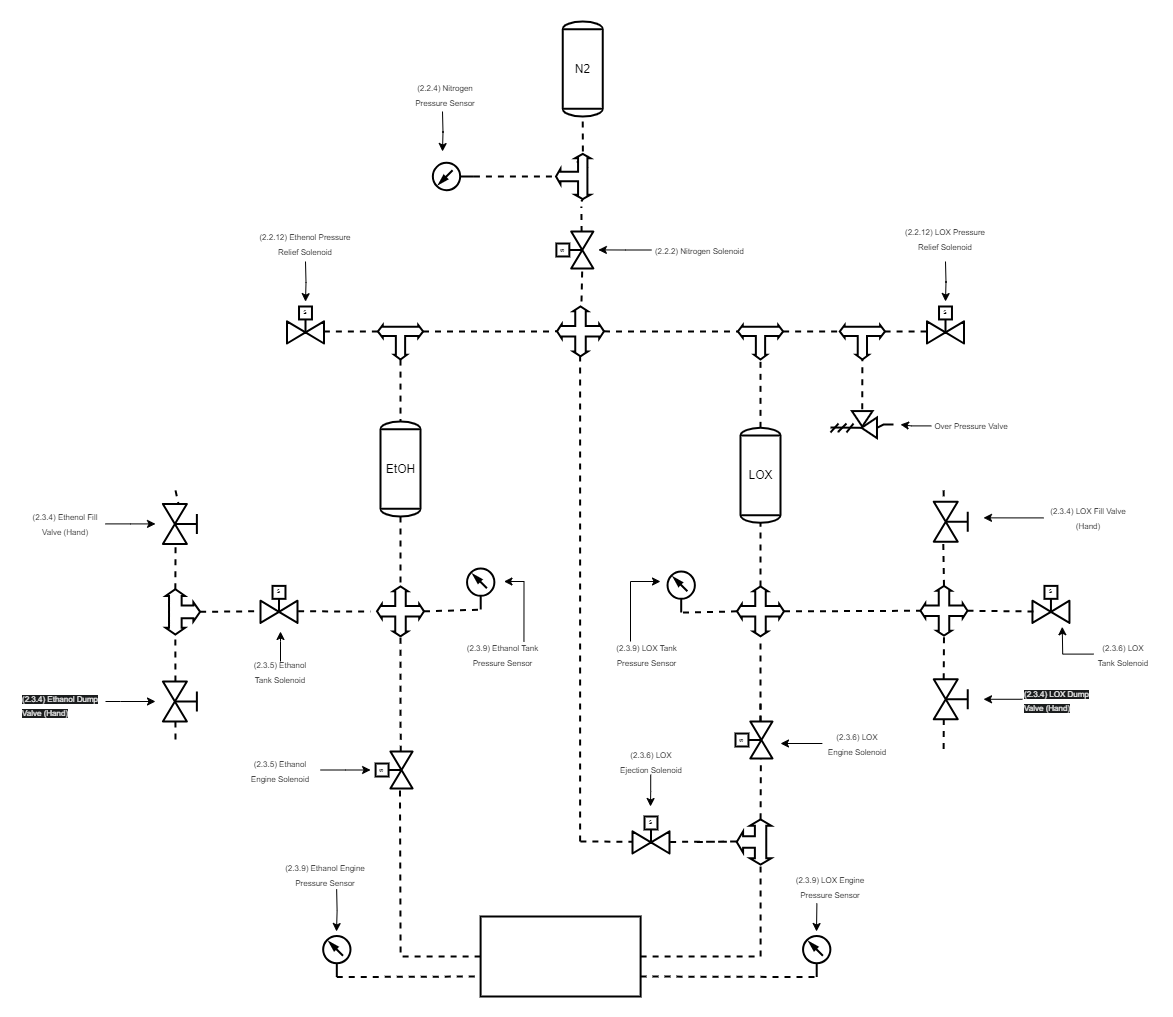
\includegraphics[width=1\textwidth]{figures/fluidplan3_electrical_draft2.png}
            \caption{A simplified diagram of the fluid system showing valves and sensors that interface with the electronics.}
            \label{fig:fluid_elec}
        \end{figure}

    \subsubsection{State Diagram}

        \begin{figure}[H]
            \centering
            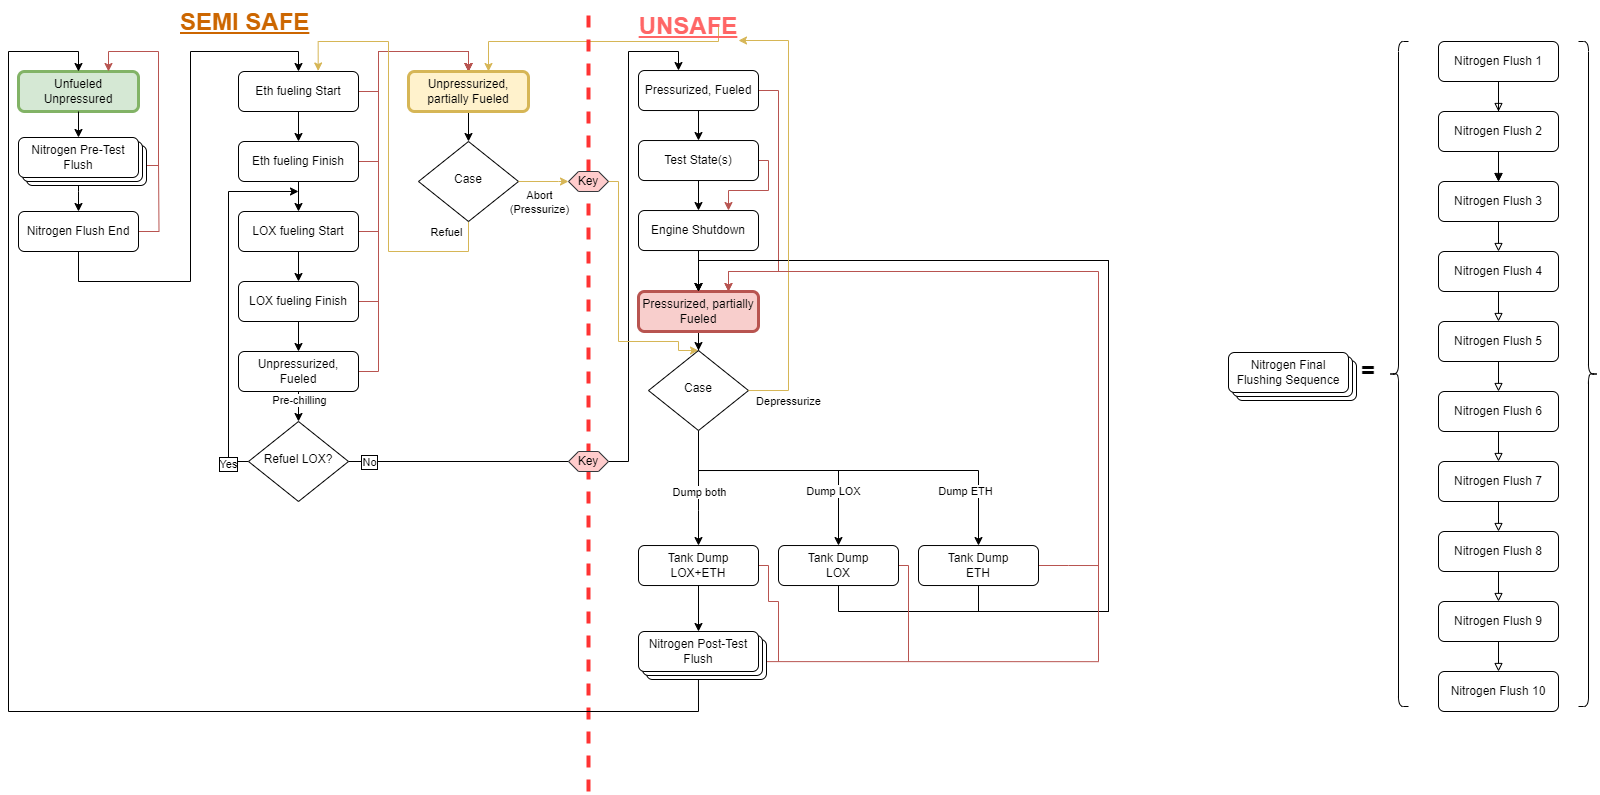
\includegraphics[width=1\textwidth]{figures/Fluid_States_blockdiagram_v3.png}
            \caption{A diagram showing the unsafe and semi-safe fluid system control states.}
            \label{fig:state_diagram}
        \end{figure}

        A state diagram (shown in figure \ref{fig:state_diagram}) was generated to show the different states that the fluid system should have, as well as the states that are available for transitioning from any given state. Sates are sorted into "unsafe" and "semi-safe". Unsafe states can be forced to transition into specific semi-safe states at any time by the test operator using an emergency-stop, or automatically if unsafe conditions are detected by the sensors. For a full list of state definitions see appendix \ref{appendix:valve_states_table}.
        % Do we also want to include the state table with the states of each of the valves?

    \subsubsection{System Overview}

        A generalized diagram of the test stand electronics system is shown in figure \ref{fig:gen_elec}. Signal inputs to a controller include a serial data link with the test operator, pressure sensor values, temperature sensor values, and the output of an E-stop located at the test bench within reach of the test operator. Controller outputs include the test bench serial link and digital valve state signals that are used to drive the solenoid valves in the engine fluid system. Drivers, either a set of relays or solid state switches, are used to "switch" the 24V power supply voltage to the solenoid valves based on the valve state signals from the controller. A 24V power supply with a power rating of greater than 500W is needed in order to supply enough current for all solenoid valves. Since it is unlikely that any power outlets will be available at the test site, this will likely be a portable battery power supply. Integrated charging from additional solar arrays is one feature of many such supplies that could be useful in this case. DC/DC converts are used to create lower voltages for powering the controller, sensors, and sensor interfaces from the primary 24V supply.

        \begin{figure}[H]
            \centering
            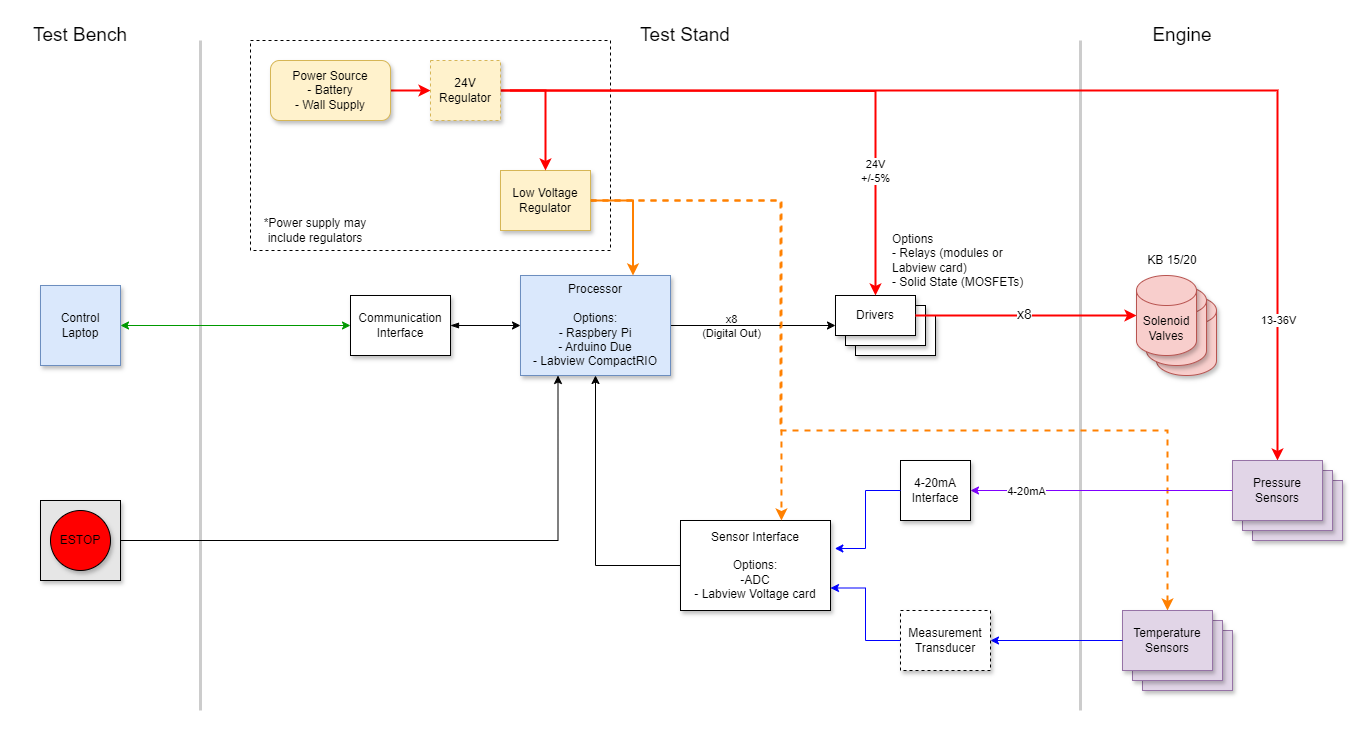
\includegraphics[width=1\textwidth]{figures/Electronics_Diagram_General.png}
            \caption{A general diagram of the test stand electronics system and interface to the test operator and engine.}
            \label{fig:gen_elec}
        \end{figure}

        A few options for the controller have been identified, each with its own advantages and disadvantages. These options are under consideration:
        \begin{itemize}
            \item Arduino Due
            \item Raspberry Pi 5B
            \item National Instruments CompactRIO Controller
        \end{itemize}

        For the Arduino Due or Raspberry Pi, a multi-channel \ac{ADC} and set of amplifiers can be used to convert raw sensor output signals into digital signals read by the controller. Although both options include on-board ADCs, an external ADC can allow for higher sample rates and resolution, while the amplifiers adjust the bias and full-scale voltage range of the analog signals going into the ADC. A 4-20mA interface is needed to convert the current signals (in the range of 4 to 20mA) from the pressure sensors into a voltage that is read by the ADC. A high-accuracy resistor with sufficient power rating can be used for this, as current sensors tend to have lower accuracy. If the CompactRIO Controller is used, the sensor interface will consist of the appropriate I/O \ac{DAQ} modules available from NI, as listed above. The NI CompactRIO LabVIEW system is preferred as it is modular, tested, and robust, however it is much more expensive than an Arduino or Raspberry Pi-based system. If sufficient funding for a LabVIEW-based system is not available, the Arduino Due is preferred to a Raspberry Pi since it does not have overhead tasks like the Pi operating system.

    \subsubsection{Fault Tolerance}

        Safety is of utmost concern in this system. A semi-redundant architecture (shown in figure \ref{fig:safe_elec}) includes a primary controller, as described above, and a secondary controller with a more limited number of states. The primary controller is monitored with a watchdog timer. If this fails in a detectable way: either in a latched state, or completely non-functional with all outputs set low, control is swapped to the secondary controller which is waiting in the safe state. This "swap" is executed using a latch (labeled the "State Latch") which controls a set of multiplexors that select the active controller's valve state signals and pass them along to the solenoid drivers. While only one controller is in control of the valve states at any time, both controllers are always reading the sensor data. The latch can only switch from the primary controller to the secondary one, and not back to the primary. This ensures that a failed primary controller is not given control again.
        
        The second controller operates with a more limited state machine that does not include the test mode or any mode that is not classified as safe. Its role is to pass along sensor data to the operator and to provide a means of transitioning to other safe sates. It has its own watchdog time that ensures it is available in the event of a failure of the primary controller. The intention here is to avoid a brief transition into an unpowered state in the time between failure occurrence and failure detection, then a transition back into the test state once control has been swapped, which could be dangerous. Therefore, the watchdog timers must also have a timing window shorter than the engagement time of the valves. Each controller has an independent communication link to the test bench, with dedicated data displays so that both can be monitored in real-time by the test operator.

        \begin{figure}
            \centering
            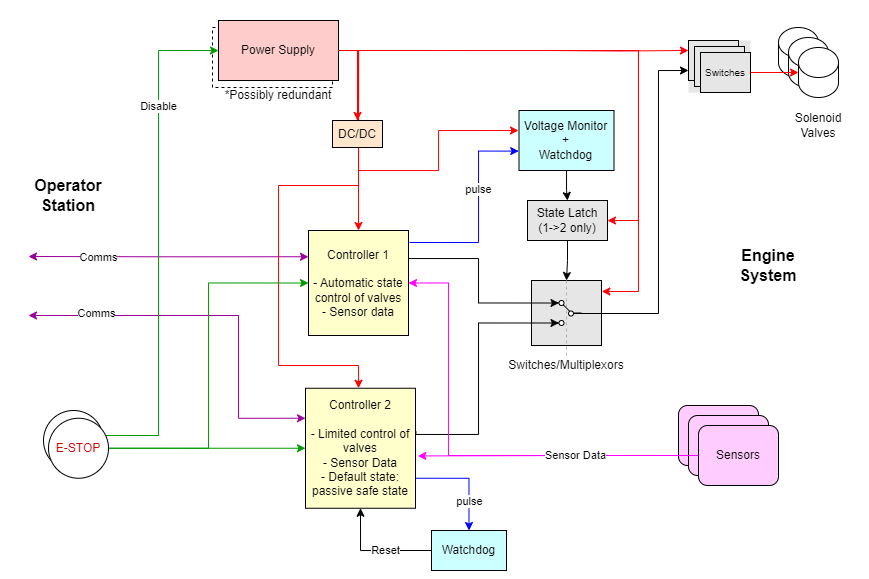
\includegraphics[width=1\textwidth]{figures/Electronics_Safety_Architecture_Draft2.png}
            \caption{A diagram showing the safety architecture for the electronics system.}
            \label{fig:safe_elec}
        \end{figure}

